\documentclass[aspectratio=1610]{beamer}
%Information to be included in the title page:

\usetheme{Madrid}
%%%%%%%%%%%%%%%%%%%%%%%%%%%%%%%%%%%
%% DO NOT CHANGE

\usetheme{default}
\useinnertheme{circles}
\useoutertheme{infolines}
\usefonttheme{serif}

\usepackage{etoolbox}

%% T for navigation symbols
%%\setbeamertemplate{navigation symbols}{}

%% T for header
%% \setbeamertemplate{headline}{%
%%   \leavevmode%
%%   \ifdefempty{\insertsubsectionhead}{
%%     \begin{beamercolorbox}[wd=0.99\paperwidth,ht=2.25ex,dp=1ex,center]{section in head/foot}%
%%       % \hbox to .5\paperwidth{\hfil\insertsectionhead\hfil}
%%       \insertsectionhead
%%     \end{beamercolorbox}%
%%   }{
%%     \begin{beamercolorbox}[wd=.44\paperwidth,ht=2.25ex,dp=1ex,right]{section in head/foot}%
%%       % \hbox to .5\paperwidth{\hfil\insertsectionhead\hfil}
%%       \insertsectionhead
%%     \end{beamercolorbox}%
%%     \begin{beamercolorbox}[wd=.1\paperwidth,ht=2.25ex,dp=1ex,center]{section in head/foot}%
%%       % \hbox to .5\paperwidth{\hfil\insertsectionhead\hfil}
%%       -
%%     \end{beamercolorbox}%
%%     \begin{beamercolorbox}[wd=.44\paperwidth,ht=2.25ex,dp=1ex,left]{subsection in head/foot}%
%%       % \hbox to .5\paperwidth{\hfil\insertsubsectionhead\hfil}
%%       \insertsubsectionhead
%%     \end{beamercolorbox}
%%   }%
%% }

%% T for frame title
\setbeamertemplate{frametitle}{%
  \usebeamerfont{frametitle}\insertframetitle\strut%
  \vskip-0\baselineskip%
  \leaders\vrule width .95\paperwidth\vskip1pt%
  \vskip0pt%
  \nointerlineskip
}

%% T for footer
\setbeamercolor{footlinecolor}{fg=cyan,bg=green}
\setbeamercolor{author in head/foot}{fg=blue}

\setbeamertemplate{footline}{%
  \leavevmode%
  \hbox{%
  \begin{beamercolorbox}[wd=.26\paperwidth,ht=2.25ex,dp=1ex,left]{author in head/foot}%
    \hspace*{2ex}\usebeamerfont{author in head/foot} Dept. CSE, UT Arlington
  \end{beamercolorbox}%
  \begin{beamercolorbox}[wd=.50\paperwidth,ht=2.25ex,dp=1ex,center]{author in head/foot}%
    \usebeamerfont{title in head/foot}Scalable Modeling \& Imaging \& Learning Lab (SMILE)
  \end{beamercolorbox}%
  \begin{beamercolorbox}[wd=.24\paperwidth,ht=2.25ex,dp=1ex,right]{date in head/foot}%
    \usebeamerfont{date in head/foot}
    \insertshortdate{}\hspace*{1em}  % date
    \insertframenumber/\inserttotalframenumber\hspace*{2ex}
  \end{beamercolorbox}}%
  \vskip0pt%
}
%%%%%%%%%%%%%%%%%%%%%%%%%%%%%%%%%%%%%%%%%%%%%%%%

\title{Sample title}
\author[Gcc]{Dingchao Gao}
\institute[ISCAS]{Institute of Software Chinese Academy of Sciences}

\begin{document}

\begin{frame}[plain]
  \titlepage
  %  Title page
\end{frame}
\section{induction}
\begin{frame}
  SIS, 
\end{frame}

\section{example}
\begin{frame}{problem}
  \begin{figure}[htbq]
    \centering
    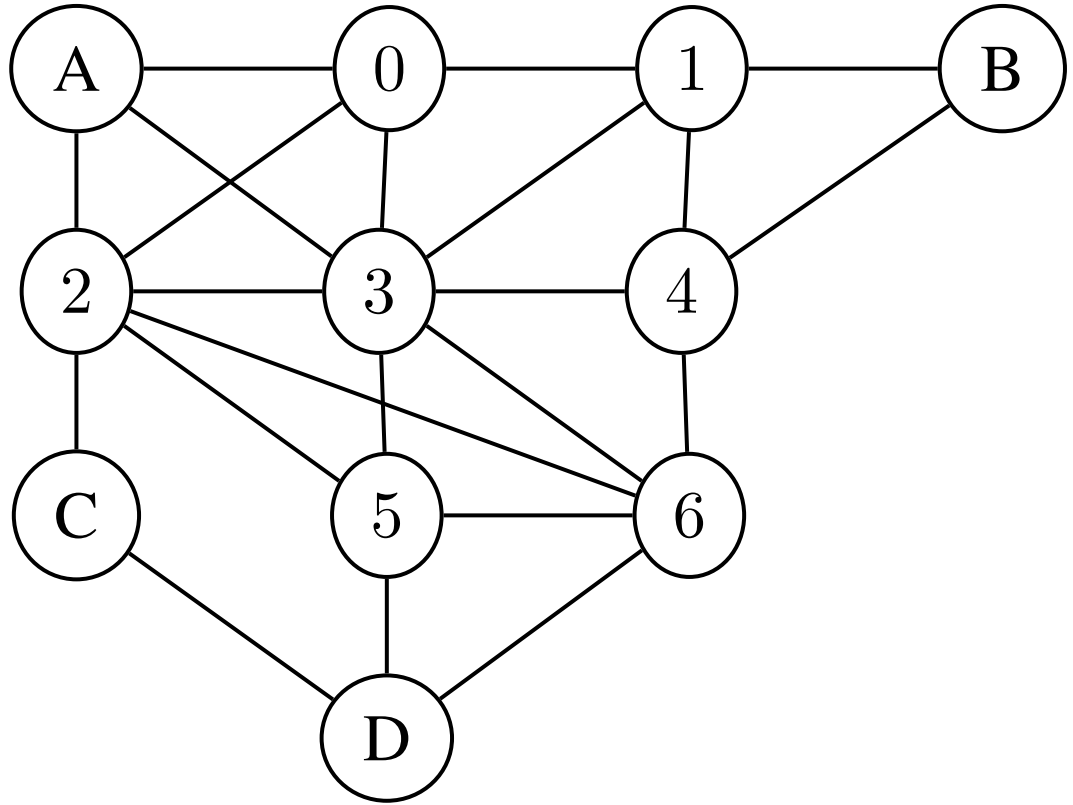
\includegraphics[width=0.5\textwidth]{figure/problem.png}
    \caption{Zed city as an undirected graph} 
    \label{fig-zed}
  \end{figure}
\end{frame}
\begin{frame}[fragile]
  \frametitle{boolean function}
  \begin{columns}
    \begin{column}{0.45\linewidth}
      \begin{block}{python implementation of f }
        \begin{lstlisting}[language=Python]
def f(v0, ..., v6 : BitVec(2)) -> BitVec(1):
  c0 = (v0 != ’00’)
  c1 = (v1 != ’01’) and (v1 != v0)
  c2 = (v2 != ’00’) and (v2 != ’10’) and (v2 != v0)
  c3 = (v3 != ’00’) and (v3 != v0) and (v3 != v1) and (v3 != v2)
  c4 = (v4 != ’01’) and (v4 != v1) and (v4 != v3)
  c5 = (v5 != ’11’) and (v5 != v2) and (v5 != v3)
  c6 = (v6 != ’11’) and (v6 != v2) and (v6 != v3) and (v6 != v4) and (v6 != v5)
  return c0 and c1 and c2 and c3 and c4 and c5 and c6
          \end{lstlisting}
      \end{block}
    \end{column}
    \begin{column}{0.45\linewidth}
      \begin{block}{hand-optimized python implementation of f }
        \begin{lstlisting}[language=Python]
def f(v0, ..., v6 : BitVec(2)) -> BitVec(1):
  c1 = (v1[0] == v1[1]) and (v3 != v1)
  c023 = ((v0 ˆ v2 ˆ v3) == ’00’)
  c4 = (v4 != v1) and (v4 != v3)
  c5 = (v5 != v2) and (v5 != v3)
  c6 = ((v2 ˆ v3 ˆ v5 ˆ v6) == ’00’) and (v6 != v4)
  return c1 and c023 and c4 and c5 and c6
          \end{lstlisting}
      \end{block}
    \end{column}
  \end{columns}
\end{frame}

\begin{frame}{flow\footfullcite{example}}
  \begin{itemize}
    \item Angel:prepare a uniform quantum state
    given as input a Boolean function
    \item Tweedledum:synthesizing,
    manipulating, and optimizing quantum circuits
    \item Caterpillar:automatically translate the combinational parts of a quantum
    algorithm into quantum gates
  \end{itemize}
\end{frame}
\begin{frame}{initial state\footfullcite{initial}}
  \begin{itemize}
    \item formal here
  \end{itemize}
\end{frame}
\begin{frame}{initial state}
  figure here
\end{frame}
\begin{frame}{initial state example}
  \begin{itemize}
    \item for
    \item figure
  \end{itemize}
\end{frame}

\begin{frame}{compiling oracle}
  \begin{itemize}
    \item 
  \end{itemize}
\end{frame}
\begin{frame}{XAG\footfullcite{multiplicative}}
  \begin{itemize}
    \item change a for b
    \item figure
  \end{itemize}
\end{frame}
\begin{frame}{XAG example}
  \begin{itemize}
    \item for
    \item we 
  \end{itemize}
\end{frame}
\begin{frame}{result}
  table   
\end{frame}

\section{tweedledum}
\begin{frame}{induction}  
  ABC 
\end{frame}
\begin{frame}{compilation flow}
  \begin{figure}[htbq]
    \centering
    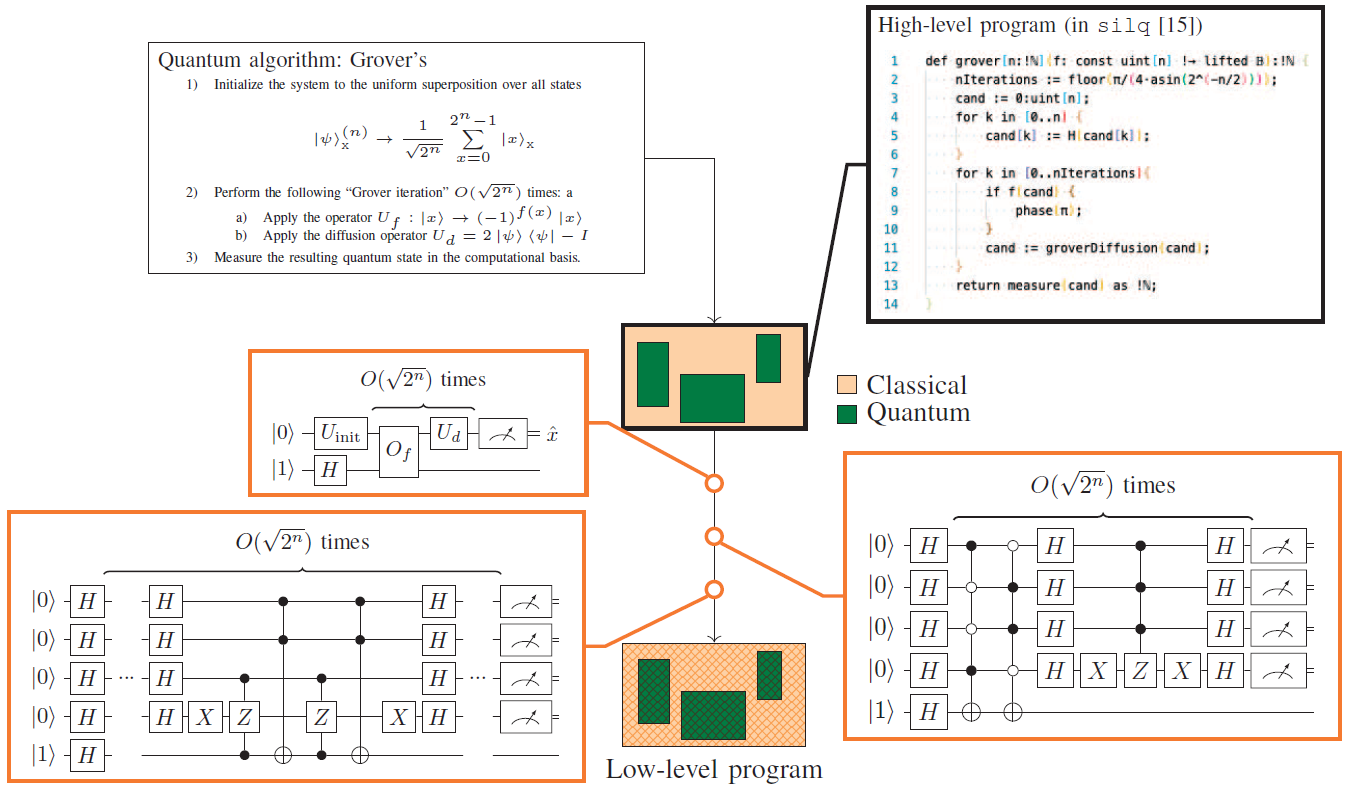
\includegraphics[width=0.8\textwidth]{figure/work_flow.png}
    \caption{compilation flow overview} 
    \label{fig-compilation}
  \end{figure}
\end{frame}
\begin{frame}{flexibility}
  \begin{figure}[htbq]
    \centering
    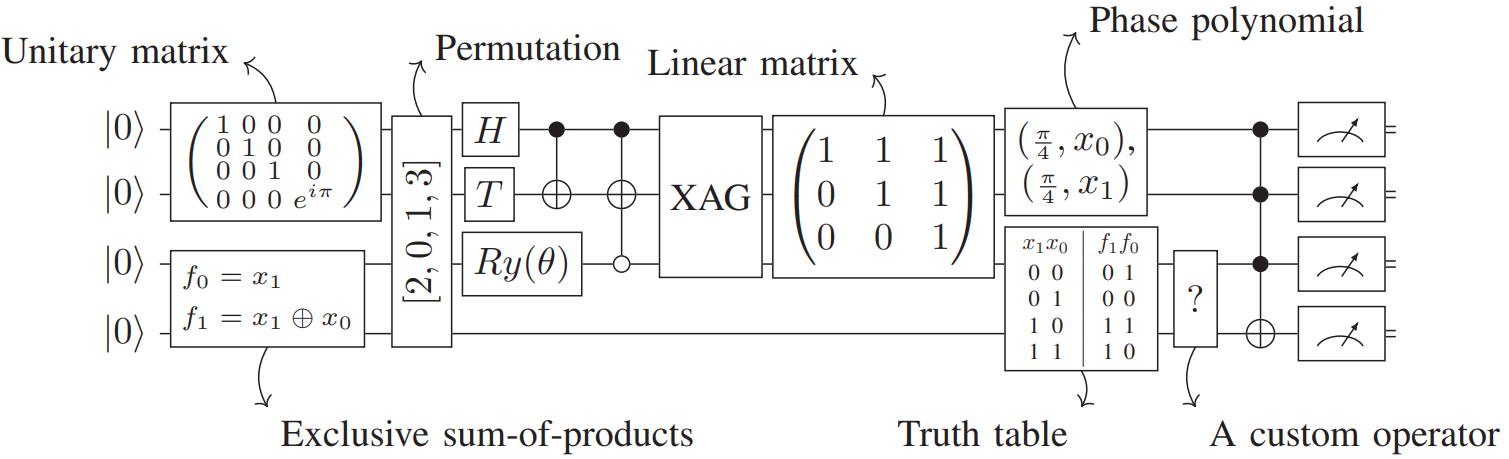
\includegraphics[width=0.9\textwidth]{figure/flex.png}
    \caption{tweedledum's IR flexibility} 
    \label{fig-flex}
  \end{figure}
\end{frame}
\begin{frame}{synthesis}
  \begin{itemize}
    \item 
  \end{itemize}  
\end{frame}
\begin{frame}{synthesis}
  \begin{figure}[htbq]
    \centering
    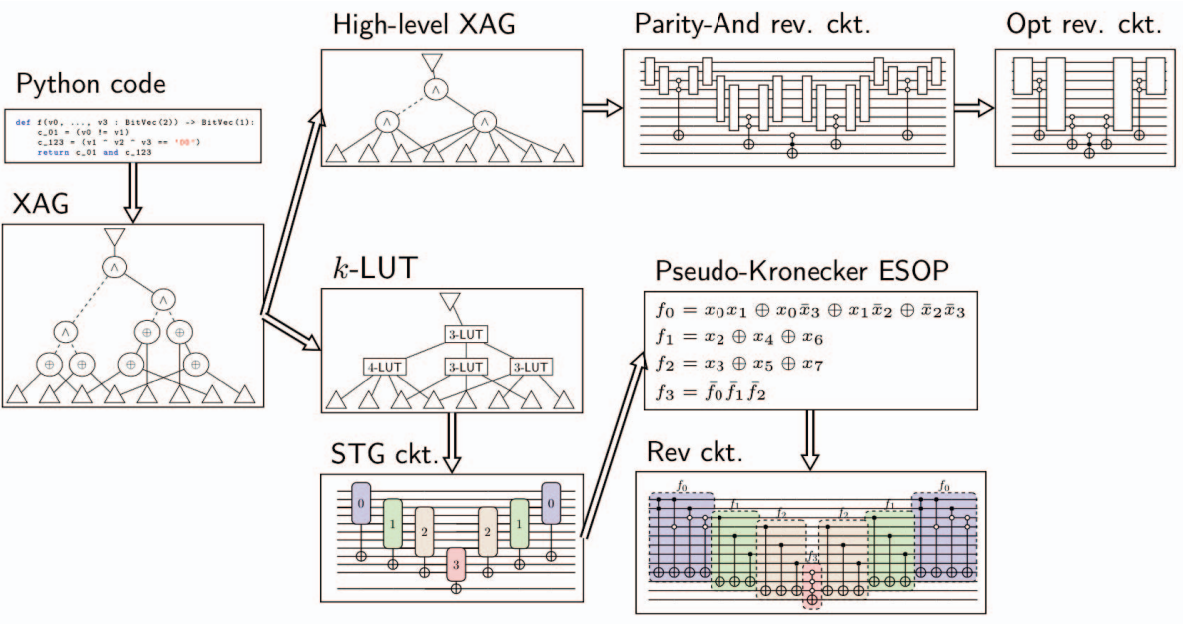
\includegraphics[width=0.7\textwidth]{figure/boolean.png}
    \caption{overview of possible Boolean function synthesis flows} 
    \label{fig-boolean}
  \end{figure}
\end{frame}
\begin{frame}{compilation passes}
  \begin{itemize}
    \item 
  \end{itemize}
\end{frame}
\section*{}
\begin{frame}[noframenumbering,allowframebreaks,t]
	\frametitle{references}
	\printbibliography
\end{frame}
\begin{frame}
\centering
\Huge{END\\Thank you}
\end{frame}
\end{document}